%-----------------------------------------------------%
% Quizz Module 1										
%-----------------------------------------------------%
% Attention il n'y que les questions par l'environnement
% Quizz

\documentclass[12pt, LuaLaTeX]{article}
\usepackage{moodle}
\usepackage{ae}
\usepackage{graphicx}


\usepackage{fontspec}
\setmainfont{Arial}

%-----------------------------------------
% Module QuizzMoodle in MAGIC path
%-----------------------------------------
% Need : \edxlibspath defined


%-----------------------------------------
% Define counter for question

\newcounter{uQuizznum}
\renewcommand\theuQuizznum{\arabic{uQuizznum}}
\newcommand{\uQuizznum}{\stepcounter{uQuizznum}ID\theuQuizznum}

\setcounter{uQuizznum}{0}
\newcommand\QuizzIDprefix{no-prefix}
\newcommand\QuizzName{no-name}

\newcommand{\QuizzID}{\QuizzIDprefix-\uQuizznum}

%\usepackage[french]{babel}
%\usepackage[utf8]{inputenc}
%\usepackage[T1]{fontenc}
%\usepackage{lmodern}


\def\QuizzName{Module1}
\def\QuizzIDprefix{Q-\QuizzName}

\title{Auto-Quizz Magic}
\author{\QuizzName}

\begin{document}

\maketitle

\begin{quiz}{\QuizzName}
 	
\begin{multi}[multiple=true]{\QuizzID}
	Entourer les attaques généralement de type  ciblée :\\
	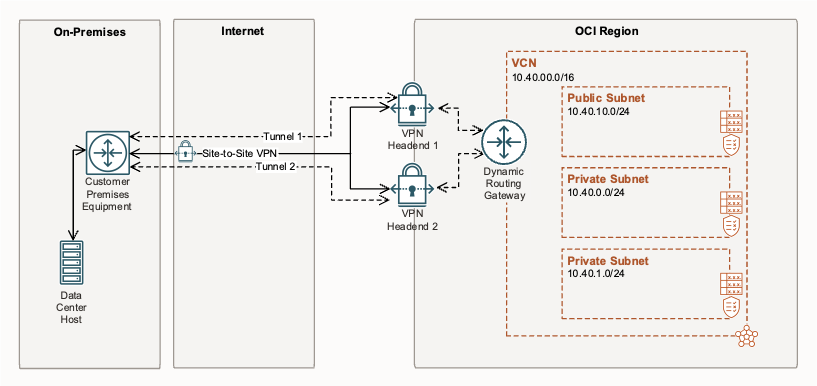
\includegraphics[scale=0.5]{pictures/image.png}
	
\item 	Phishing ou hameçonnage
\item 	Ransomware ou rançongiciel
\item* 	Social engineering ou ingénierie sociale
\item* 	Spear phishing ou l'arnaque au président
\end{multi}

\begin{multi}[multiple=true]{\QuizzID}
	Entourer les attaques généralement de type  ciblée :
\item 	Phishing ou hameçonnage
\item 	Ransomware ou rançongiciel
\item* 	Social engineering ou ingénierie sociale
\item* 	Spear phishing ou l'arnaque au président
\end{multi}

\begin{multi}[multiple=true]{Cyberedu-QUIZZ-ID-1.20}
	Lors de la création du site Web de notre association étudiante, si vous stockez les informations suivantes pour chaque membre : nom, prénom, adresse, adresse email. Auprès de quel organisme devez-vous faire une déclaration (Voir ANSSI \url{https://www.ssi.gouv.fr/administration/formations/cyberedu/contenu-pedagogique-cyberedu/} Slide n° 60 - 64 : Droit de protection des données à caractère personnel)?
\item 	Gendarmerie
\item 	Université
\item* 	CNIL
\item 	Hadopi
\end{multi}
   	
 \end{quiz}

\end{document}
